%%%%%%%%%%%%%%%%%%%%%%%%%%%%%%%%%%%%%%%%%%%%%%%%%%%%%%%%%%%%%%%%%%%%%%%%
%                                                                      %
%     File: Thesis_Background.tex                                      %
%     Tex Master: Thesis.tex                                           %
%                                                                      %
%     Author: Andre C. Marta                                           %
%     Last modified :  4 Mar 2024                                      %
%                                                                      %
%%%%%%%%%%%%%%%%%%%%%%%%%%%%%%%%%%%%%%%%%%%%%%%%%%%%%%%%%%%%%%%%%%%%%%%%

\chapter{Computational Methods}
\label{chapter:computational_methods}

After accessing theory in previous chapter, in this chapter it is explained how the computational methods used in this thesis. The chapter stars by definig the dynamic integration method used to solve the equations of motion, Sec. \ref{sec:runge-kutta}, followed by the description of the numerical methods used to integrate the \gls{bet} equations, Sec. \ref{sec:blade_integration} .

In sequence the flowchart of the aglorithm used to solve the problem, Sec. \ref{sec:flow_chart}, where a detailed explanation of the routine is done. Also it is presented the Matlab application developed to help visualize and interact easier with the simulation inputs, Sec. \ref{sec:application_interface}.

Finally, in this chapter the validation and verification is done, Sec. \ref{sec:validation_verification}, using experimental and simulation a set of experimental tests are used to understand both the rotor model and the dynamic behaviour. As a last step, the mesh study is conducted to optimize the time consumption for further simulations in Sec. \ref{sec:mesh_study}.

\section{Numerical Integration}

As other mechanical or electrical systems, the autorotation problema is a classical \gls{ode} problem. To solve the system equations of motion, Eq. \ref{eq:force_equation} and Eq. \ref{eq:momentum_equation}, it is necessary to integrate the equations in time. In this form, the vehicle's are given by a non-linear system of \gls{ode} and can be solve using a classical \gls{ode} time-integration method \cite{arnold_numerical_2011, press_numerical_2007, lindfield_numerical_2019}.

On other hand, the \gls{bet} is a 2D aifoil descritization method to compute rotor's forces and moments, and no function is able to define the blade's load distributions. In this way, to compute the rotor's forces and moments an integration method is used to integrate with the \gls{bet} equations, Eq. \ref{eq:total_rotor_force_rotor_frame} and Eq. \ref{eq:total_rotor_torque_rotor_frame}.

\subsection{4th Order Runge-Kutta for Vehicle Dynamics}
\label{sec:runge-kutta}

One of the most common methods is the Euler Method, defined in Eq. \ref{eq:euler_method},

\begin{equation}
    \phi_{n+1} = \phi_n + \Delta t \cdot f(\phi_n)
    \label{eq:euler_method}
\end{equation}

where $n$ is the time step number, $\phi_n$ is the state vector at the $n$-th step and $\Delta t$ is the time step, which advances from the solution at instante $t_n$ to the solution at instante $t_{n+1}$. For the presented problem, this method is not suitable once it has two key disadvantages \cite{press_numerical_2007}:

\begin{enumerate}
    \item \textbf{Accuracy}: The Euler method is not very accurate when compared with other methods, specially when large varitions of the dynamic systems occur, for the same step size \cite{press_numerical_2007}. For the current problem this means that one the rotor opens, the loads are instantaneously generated, 
    \item \textbf{Stability}: The method does not show good stability \cite{press_numerical_2007}. The key goal of autorrotation is to control the descent velocity and performe a safe landing, if the method is not stable, the rotor's descent velocity might be never stable and the rotor will not be well computed.
\end{enumerate}

Looking back to \ref{eq:force_equation} and Eq. \ref{eq:momentum_equation}, both can be writen in a general \gls{ode} form as in Eq. \ref{eq:general_ode}.

\begin{equation}
    \frac{\mathrm{d}\phi}{\mathrm{d}t} = f(t, \phi),
    \label{eq:general_ode}
\end{equation}

\noindent where $\phi$ is any variable, $t$ is the time domain and $f$ is a function that governs the change of a variable, $\phi$, over time, $t$. Solving \gls{ode} typically involves finding an solution throughout analytical methods such as separation of variables or integrating factors. However, the current set of equations, Eq. \ref{eq:force_equation} and Eq. \ref{eq:momentum_equation}, involves non-linear \gls{ode} which cannot be solved analytically. In this way, the numerical integration method must be implemented to solve the equations.

A classical numerical method for solving non-linear \gls{ode} is the Runge-Kutta mehtod \cite{arnold_numerical_2011}. The \gls{rk4} is widely used for aricraft dynamics solver \cite{ozdemir_linear_2008,milne_high-fidelity_2023,yoo_dynamics_2024} and is nowadays, commanly used to solve non-linear flight equations models for training Phycal-Informed \gls{nn} \cite{yu_aircraft_2019}.

The math scheme for solving any \gls{ode} using \gls{rk4} is presented in Eq. \ref{eq:rk4},

\begin{equation}
    \phi_{n+1} = \phi_{n} + \frac{1}{6} k_1 + \frac{1}{3} k_2 + \frac{1}{3} k_3 + \frac{1}{6} k_4 + O(h^5)
    \label{eq:rk4}
\end{equation}

\noindent where $\phi_{n+1}$ is the next time step to compute, $\phi_{n}$ is the current time step function value and $k_1$ to $k_4$ are the method coefficents computed as in Eqs. \ref{eq:rk4_k1} to \ref{eq:rk4_k4},

\begin{equation}
    k_1 = f\left(t_n, \phi_n\right) \Delta t
    \label{eq:rk4_k1}
\end{equation}
\begin{equation}
    k_2 = f\left(t_n + \frac{1}{2}\Delta t, \phi_n + \frac{1}{2} k_1\right) \Delta t
\end{equation}
\begin{equation}
    k_3 = f\left(t_n + \frac{1}{2}\Delta t, \phi_n + \frac{1}{2} k_2\right) \Delta t
\end{equation}
\begin{equation}
    k_4 = f\left(t_n + \frac{1}{2}\Delta t, \phi_n + k_3\right) \Delta t
    \label{eq:rk4_k4}
\end{equation}

\subsection{Integration Methods for Blade Loads}
\label{sec:blade_integration}

The \gls{bet} is a 2D aifoil descritization method compute a rotor's forces and moments, and no algebraic function defines the blade's loads distributions. In this way, a numerical integration method should be introduced to integrate both equations Eq. \ref{eq:total_rotor_force_rotor_frame} and Eq. \ref{eq:total_rotor_torque_rotor_frame}. 

The integration method choice shall consider the two key computational aspects previous defined: accuracy and speed. From a wide diversity of function integration methods and has a milestone improvement from Marques et al. \cite{marques_design_2024} (2024). Marques et al. \cite{marques_design_2024} used the Riemann sum to approximate the integral which has a error by excess or defect depending on the type of Riemann rule choosen. 

The Trapezoidal rule for numerical integration is a simple and efficient method for numerical integration \cite{press_numerical_2007}. It presents a quite good accuracy over The Riemann's rule once it based in the idea of creating subintervals with a trapezoidal shape connecting the function values winth a straigh line and then computing its area \cite{lindfield_numerical_2019}. Over more accurate methods, such as Simpson's rule, the Trapezoidal rule presents a easier and computationally effortless, once it does not require more than one function evaluation per subinterval \cite{arnold_numerical_2011, press_numerical_2007, lindfield_numerical_2019}. 

For the Trapezoidal rule the sum of the all the subintervals areas are the integral value in the interval. The Trapezoidal rule is defined as in Eq. 

\begin{equation}
    \int_{a}^{b}f(x)\,d x\approx\sum_{k=1}^{N}{\frac{f(x_{k-1})+f(x_{k})}{2}}\Delta x_{k}
\end{equation}

\noindent where $\Delta x_{k}=x_{k}-x_{k-1}$ can be a non-uniform grid discretization of the interval $\left[a, b \right]$. However, in the scope of this work the interval discretization, $\Delta x_{k} = \Delta x$, is uniform and constant.

The accuracy of this methodology can be analysed of the truncation error, $E$, \cite{lindfield_numerical_2019},

\begin{equation}
    E \le \frac{(a-b) M}{12} \Delta x^{2}.
    \label{eq:trap_trunc_error}
\end{equation}

\noindent where $M$ is the upper bound of $|f(x)''|$ with $x \in \left[a, b\right]$. Eq. \ref{eq:trap_trunc_error} shows that if the interval discretization is small enough, the accuracy can be quite good with a low computational cost. In other words, when the blade's 2D sections have a small width, $d_y$ the Trapezoidal rule can be used to compute the blade's loads distribution with a good accuracy.

\section{Simulator Development}


\subsection{Simulation flowchart}
\label{sec:flow_chart}

\begin{figure}[!htb]
    \centering
    \includegraphics[width=\textwidth]{Figures/comp_method/simulation_flowchart.png}
    \caption{Computational implementation flowchart}
    \label{fig:flowchart}
\end{figure}

\subsection{Application Interface}
\label{sec:application_interface}

\section{Model Validation and Verification}
\label{sec:validation_verification}

For the autorrotation model previous presented, a critical aspect of its performance is to understand the behavior of the system under different conditions. In this section, it will be discuss the validation and verification with the following strategy:

\begin{itemize}
    \item \textbf{1st step:} Validation and verification of the rotor-aerodynamic model with wind tunnel experimental data from \cite{brindejonc_design_2007}. This step consist in validate the \textit{black box} model, i.e. the calcutaion of the rotor force and torque inside the red box in on the flowchart presented in Fig. \ref{fig:flowchart}
    
    \item \textbf{2nd step:} Verification of the dynamic model with 2 sets of simlation data, one provided in \cite{marques_rocket_2022} and the another one presented in \cite{riegler_daedalus_2018}
\end{itemize}

\subsection{Axial Descent Validation and Verification with Wind Tunnel data}

Brindejonc et al. (2007) \cite{brindejonc_design_2007} conducted wind tunnel experiments to study a rotor under the autorotation phenomena. The experimental setup consisted of a 2-bladed with no pitch-flap coupling and no precone. The rotor characteristics are summed up in Table \ref{tb:geo_paper_validation}

\begin{table}[!htb]
    \centering
    \begin{tabular}{@{}lll@{}}
    \toprule
    \multicolumn{3}{c}{Rotor Geometry} \\ \midrule
    Blade number, $N_b$                   &  & 2           \\
    Rotor diameter, $R_r$ & [\unit{m}]              & 0.33        \\
    Blade span, $S_b$ & [\unit{m}]                  & 0.1524      \\
    Blade chord, $c$ & [\unit{m}]                 & 0.0287      \\
    Blade twist, $\frac{\mathrm{d}\theta}{\mathrm{d}S_b}$ & [\unit{m}]                 & 0           \\
    Blade pitch angle, $\theta$ & [\unit{\degree / m}] & -6, -8, -12 \\
    Airfoil                               &  & NACA 0010   \\ \bottomrule
    \end{tabular}\
    \caption[Wind tunnel rotor geometric characteristics]{Wind tunnel rotor geometric characteristics, \cite{brindejonc_design_2007}}
    \label{tb:geo_paper_validation}
\end{table}

Considering the wind tunnel data \cite{brindejonc_design_2007}, it is possible to simulate a set of diferente experimental test cases. {In \cite{brindejonc_design_2007} is presented two plots from which the following parameteres of the rotor state can be taken: the rotor's speed, the rotor's thrust force and wind velocity for all the differente pitch angles in Table \ref{tb:geo_paper_validation}. So, verify the rotor-aerodynamic model, the criterion used is the comparison between the simulated and experimental values is rotor's thrust force. However, for computing the rotor's perfomance, is still needed the rotor's induced velocity, which can be estimate with the Linear Momentum Theory \cite{leishman_principles_2006}

\begin{equation}
    v_i = \frac{T ^ {\frac{3}{2}}}{\sqrt{2 \rho A_r }},
\end{equation}

where $T$ is the trust force in \unit{N}, $\rho$ the air density in \unit{Kg/m^3} and $A$ the rotor's disk area in \unit{m^2}. 

To make a comparison, the thrust error is computed in percentage \unit{\%} as

\begin{equation}
    \mathrm{e} =\frac{|T_{mode} - T_{paper}|}{T_{paper}}
    \label{eq:error_exp_paper}
\end{equation}

So, from the paper, the results can be compiled into Tab. \ref{tb:results_paper_exp} where the error is computed using Eq. \ref{eq:error_exp_paper}.


\begin{table}[!htb]
    \centering
    \begin{tabular}{@{}llll|l|lll@{}}
        \toprule
        \multicolumn{4}{c|}{Paper Data \cite{brindejonc_design_2007}}       & \multicolumn{1}{c|}{Estimation} & \multicolumn{3}{c}{Present Work} \\ \midrule
        $\theta$ [\unit{\deg}] &  $V_\infty$ [\unit{m/s}] & $RPM$ & $F_z$ [\unit{N}]& $v_i$ [\unit{m/s}] & $F_z$ [\unit{N}] & $T$ [\unit{N/m}] & $e$ [\%]\\ \midrule
        -6 & -2 & 700.59 & 0.162 & -0.649 & 0.148 & 0.000 & 8.6 \\
        -6 & -4 & 1573.23 & 0.675 & -1.680 & 0.731 & 0.000 & 8.3 \\
        -6 & -8 & 3322.39 & 2.687 & -4.222 & 3.314 & 0.000 & 23.3 \\
        -8 & -2 & 619.54 & 0.127 & -0.553 & 0.106 & 0.000 & 17.1 \\
        -8 & -4 & 1370.03 & 0.451 & -1.286 & 0.504 & 0.000 & 11.6 \\
        -8 & -8 & 2791.17 & 1.701 & -3.113 & 2.166 & 0.000 & 27.4 \\
        -12 & -2 & 550.48 & 0.067 & -0.360 & 0.054 & 0.000 & 20.0 \\
        -12 & -4 & 1063.95 & 0.269 & -0.911 & 0.262 & 0.000 & 2.5 \\
        -12 & -8 & 2224.33 & 0.976 & -2.149 & 1.127 & 0.000 & 15.4 \\
        \bottomrule
    \end{tabular}
    \caption{results DATA}
    \label{tb:results_paper_exp}
\end{table}

\begin{figure}[!htb]
    \centering
    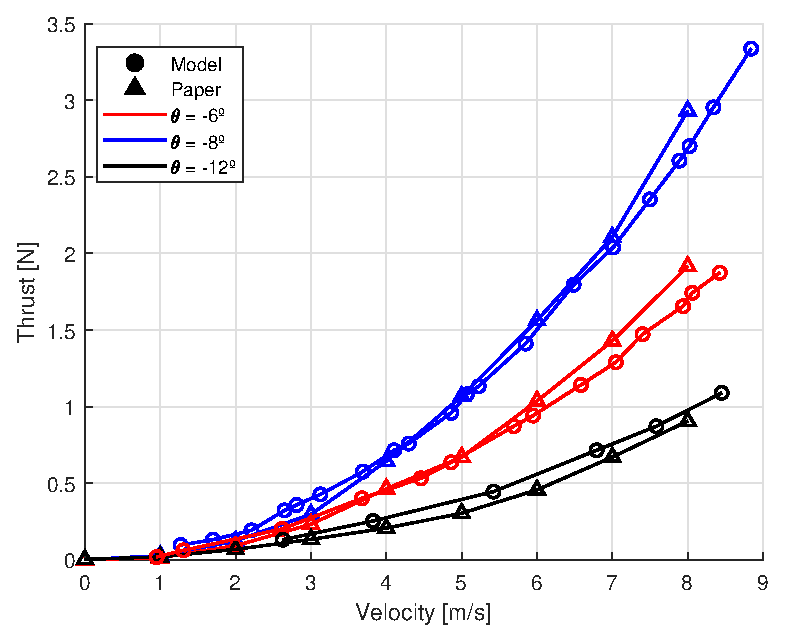
\includegraphics[width=0.5\textwidth]{Figures/comp_method/sim_B/comp_paper.eps}
    \caption{Results}
    \label{fig:comparacao_simb}
\end{figure}

For a deeper understanding of the model validity, the follow step is to make an analysis of several key variables. It was chosen the simulation number \textcolor{blue}{meter numeros na tabela e fazer uma referência}, to genera the plots that will be described next.

Starting from the velocity vectors, Eq. \ref{eq:elemets_velocity}, in the elements reference frame lets analyse each component. Fig. \ref{fig:paper_radial_velocity} presents the radial velocity component, $U_R$, which is zero once there is no horizontal plan translation of the vehicle, but the vertical component, $U_P$, present a constant value over the rotor disk area equals to the vertical descent velocity minus the induced velocity which is considered constant over the rotor's disk. 

\begin{figure}[!htb]
    \centering
    \begin{minipage}{0.49\textwidth}
        \centering
        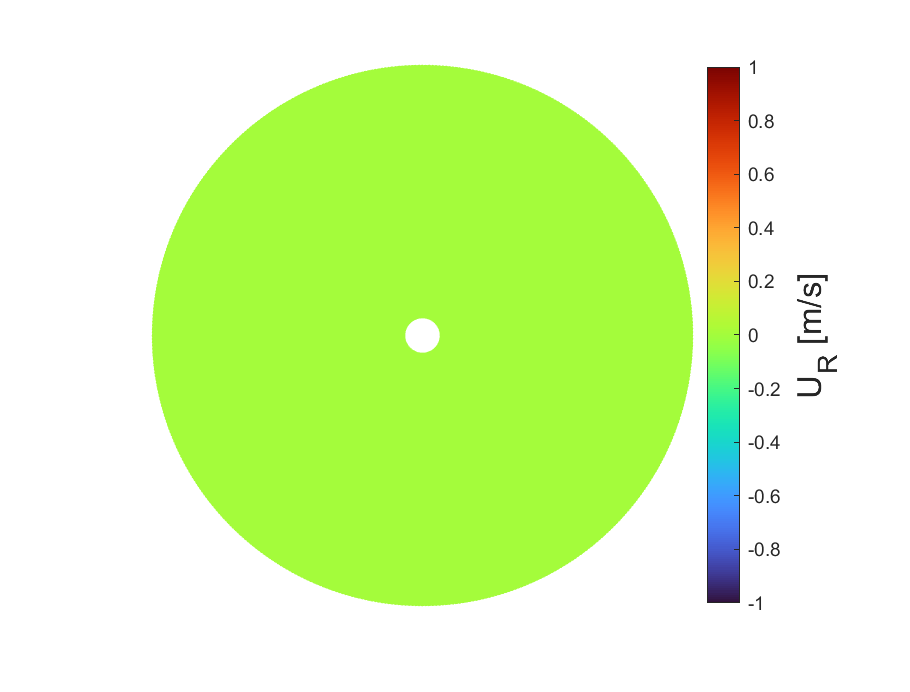
\includegraphics[width=\textwidth]{Figures/comp_method/sim_B/U_R.eps}
        \caption{Radial velocity component $U_R$}
        \label{fig:radial_velocity_paper}
    \end{minipage}%
    \hfill
    \begin{minipage}{0.49\textwidth}
        \centering
        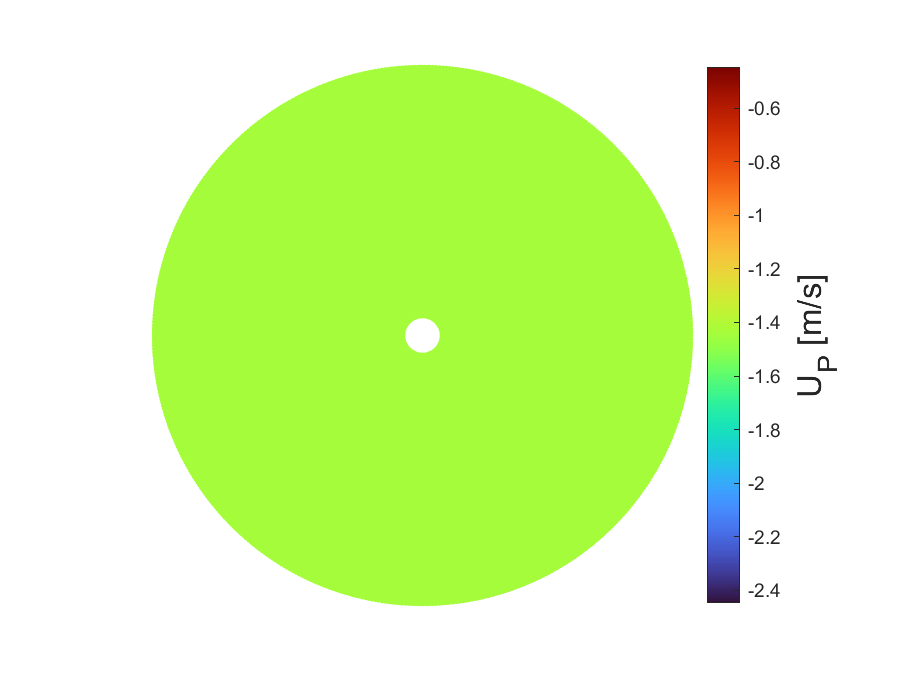
\includegraphics[width=\textwidth]{Figures/comp_method/sim_B/U_P.eps}
        \caption{Tangential velocity component $U_P$}
        \label{fig:tangential_velocity_paper}
    \end{minipage}
\end{figure} 


For the tangential velocity, $U_T$, due to rotor's rotation it is expected to has a variation over the blade length. In Fig. \ref{fig:tangencial velocity}, the tangential velocity variation can be seen, but also the axisymmetric of the rotor in terms of tangential velocity.
\begin{figure}[!htb]
    \centering
    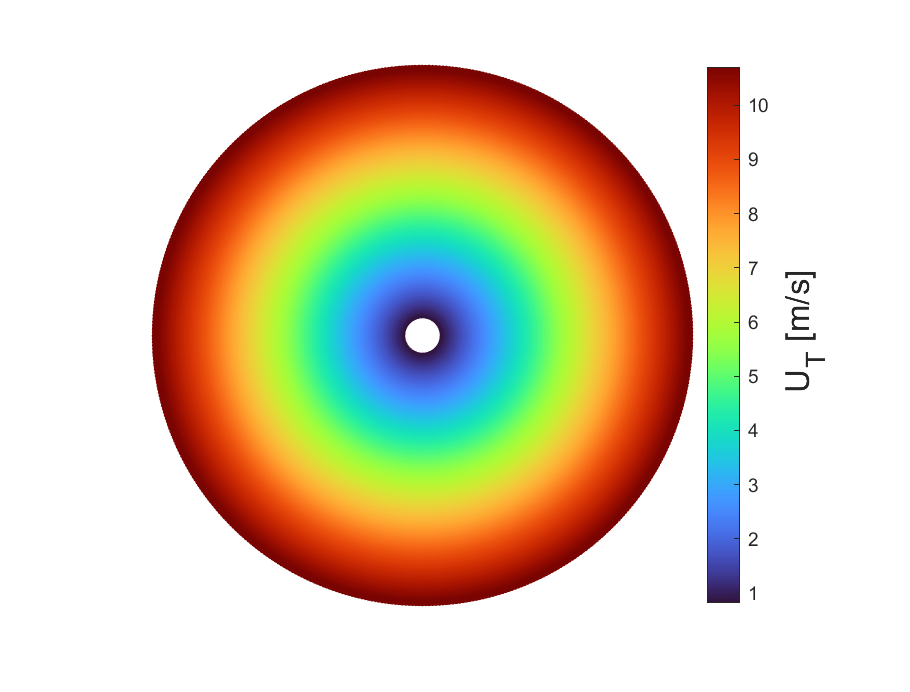
\includegraphics[width=0.49\textwidth]{Figures/comp_method/sim_B/U_T.eps}
    \caption{Axial velocity component $U_T$}
    \label{fig:axial_velocity_paper}
\end{figure}

With the velocity vector, one can look at Fig. \ref{fig:paper_incidenceangle} and check the incidence angle value over the rotor's disk with a similar axisymmetric distribution of the velocity tangential component. This distribution is expected once one looked back at Eq. \ref{eq:cosine_inflow}.

\begin{figure}[!htb]
    \centering
    \begin{minipage}{0.49\textwidth}
        \centering
        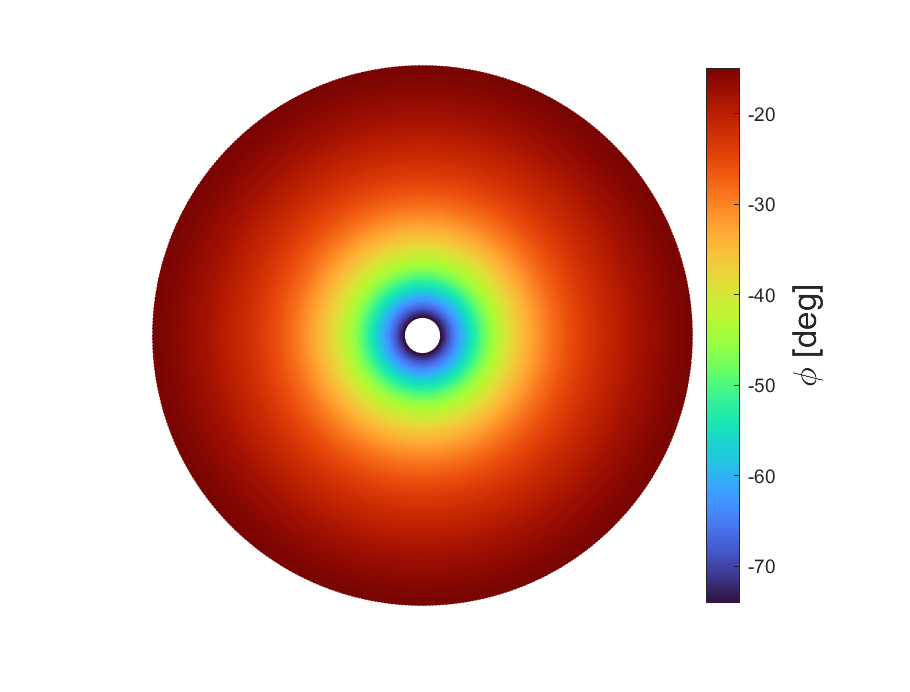
\includegraphics[width=\textwidth]{Figures/comp_method/sim_B/phi.eps}
        \caption{Blade incidence angle}
        \label{fig:blade_incidence_angle_paper}
    \end{minipage}%
    \hfill
    \begin{minipage}{0.49\textwidth}
        \centering
        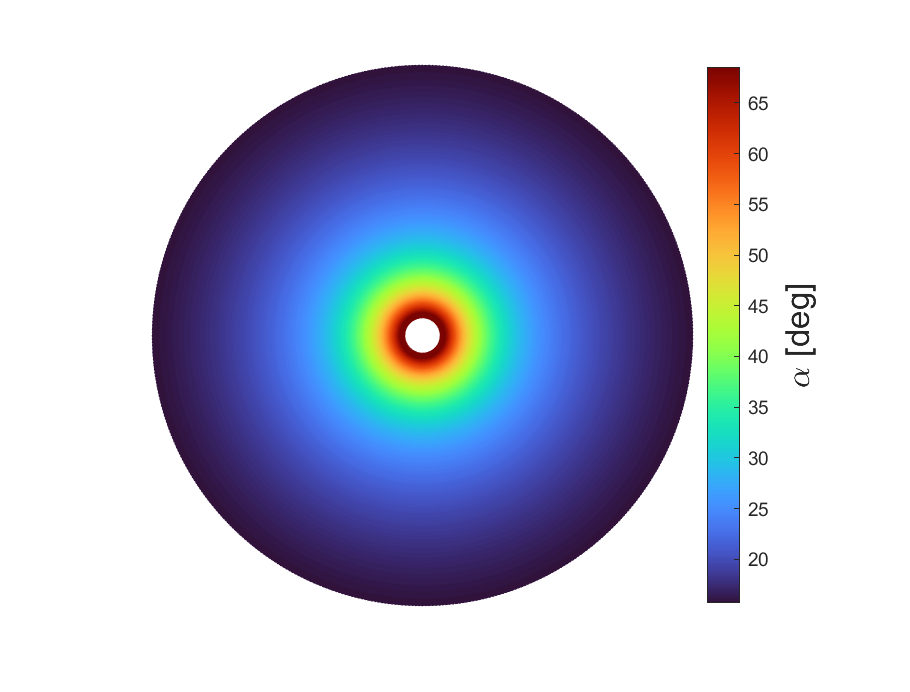
\includegraphics[width=\textwidth]{Figures/comp_method/sim_B/alpha.eps}
        \caption{Angle of attack}
        \label{fig:angle_of_attack_paper}
    \end{minipage}
\end{figure}

\begin{figure}[!htb]
    \centering
    \begin{minipage}{.49\textwidth}
      \centering
      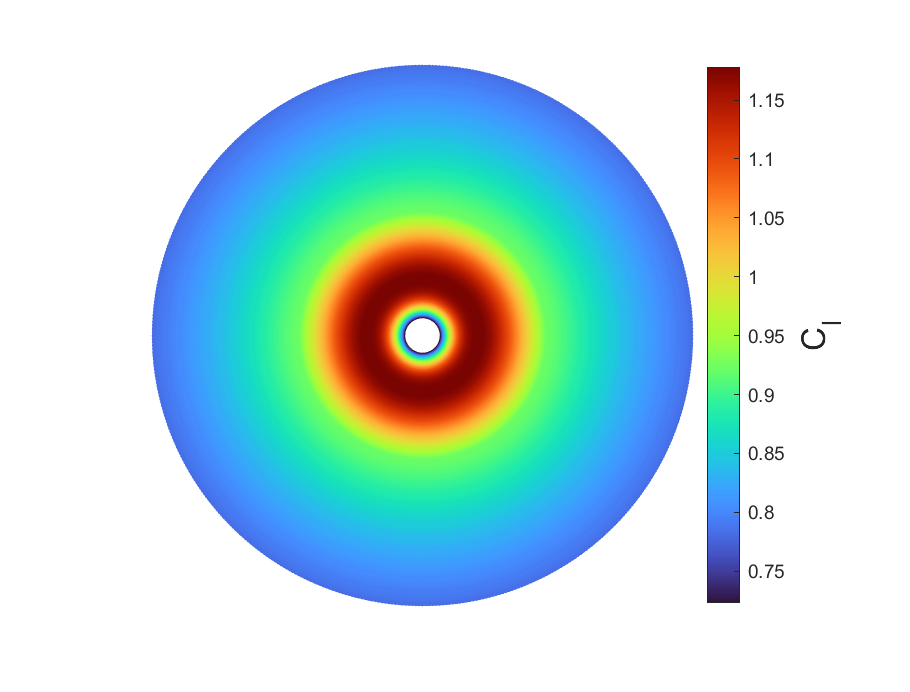
\includegraphics[width=\textwidth]{Figures/comp_method/sim_B/cl.eps}
      \caption{Lift coefficient $C_L$}
      \label{fig:lift_coefficient_paper}
    \end{minipage}%
    \hfill
    \begin{minipage}{.49\textwidth}
      \centering
      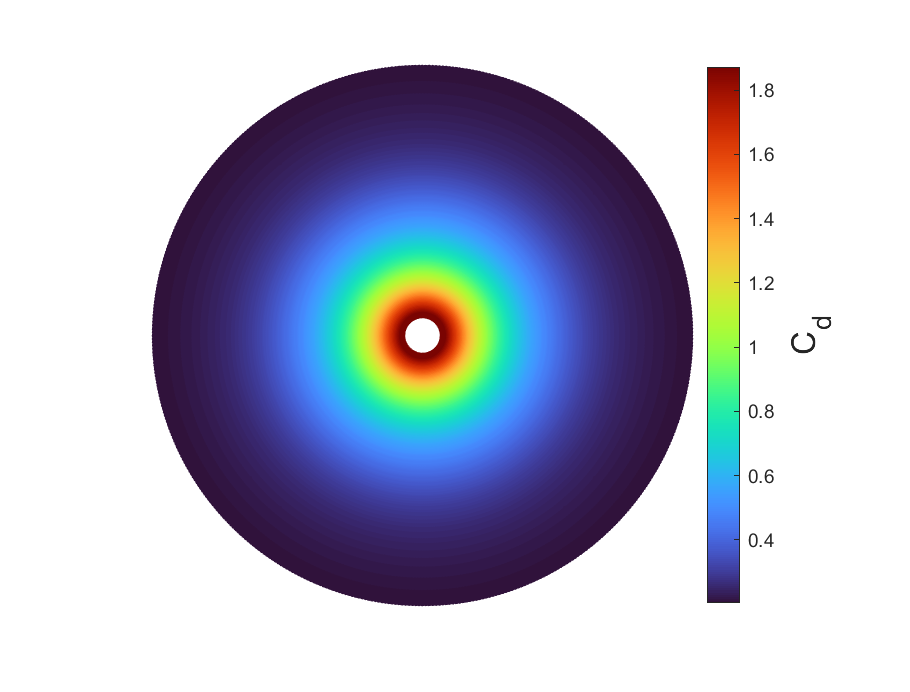
\includegraphics[width=\textwidth]{Figures/comp_method/sim_B/cd.eps}
      \caption{Drag coefficient $C_D$}
      \label{fig:drag_coefficient_paper}
    \end{minipage}
\end{figure}

\begin{figure}[!htb]
    \centering
    \begin{minipage}{.49\textwidth}
      \centering
      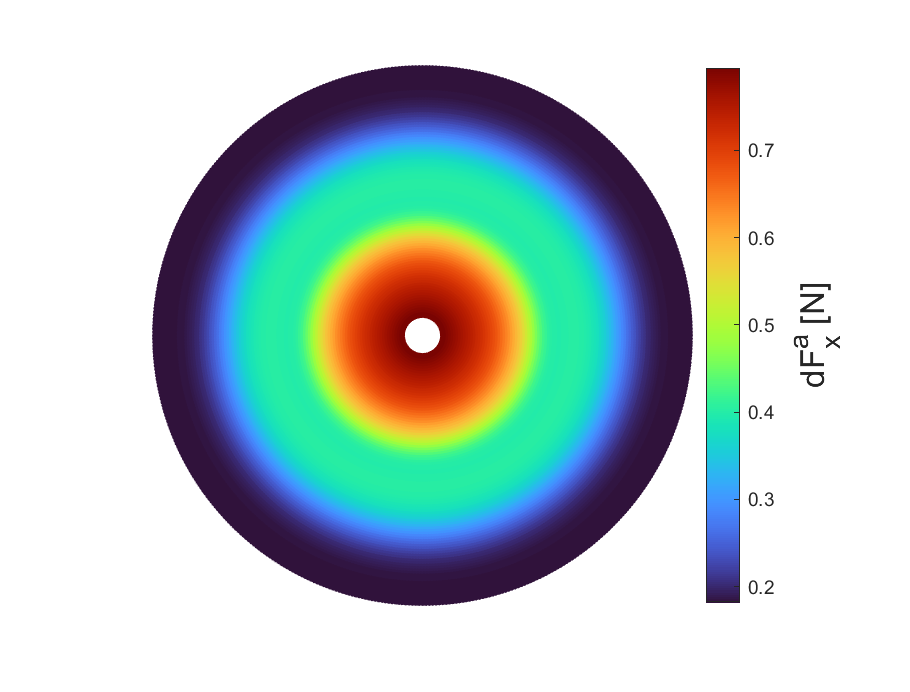
\includegraphics[width=\textwidth]{Figures/comp_method/sim_B/dFx_a.eps}
      \caption{Radial force component $F_x$ in the aerodynamic reference frame}
      \label{fig:radial_force_paper}
    \end{minipage}%
    \hfill
    \begin{minipage}{.49\textwidth}
      \centering
      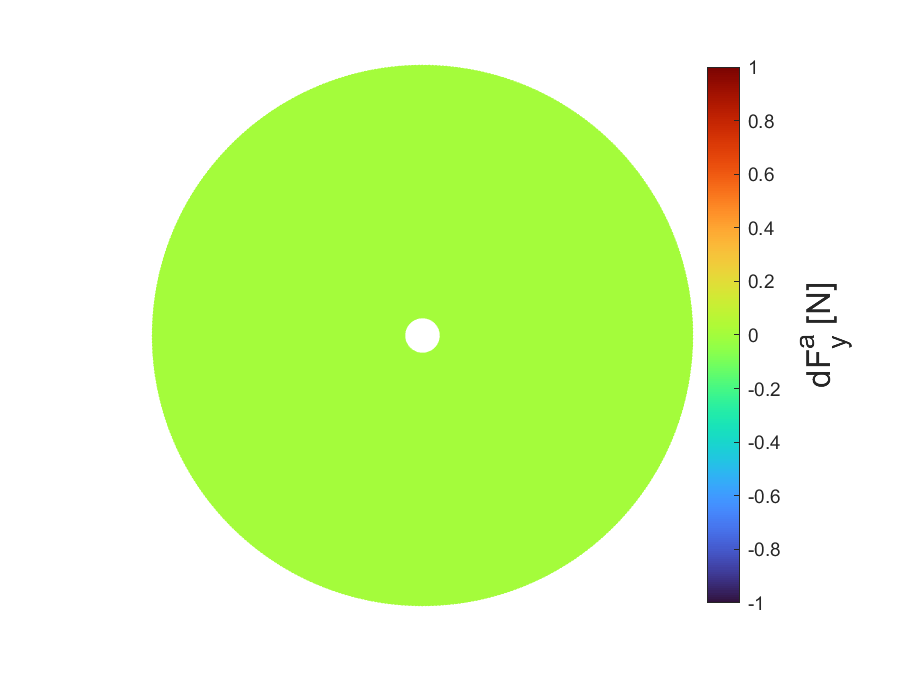
\includegraphics[width=\textwidth]{Figures/comp_method/sim_B/dFy_a.eps}
      \caption{Tangential force component $F_y$ in the aerodynamic reference frame}
      \label{fig:tangential_force_paper}
    \end{minipage}
\end{figure}

\begin{figure}[!htb]
    \centering
    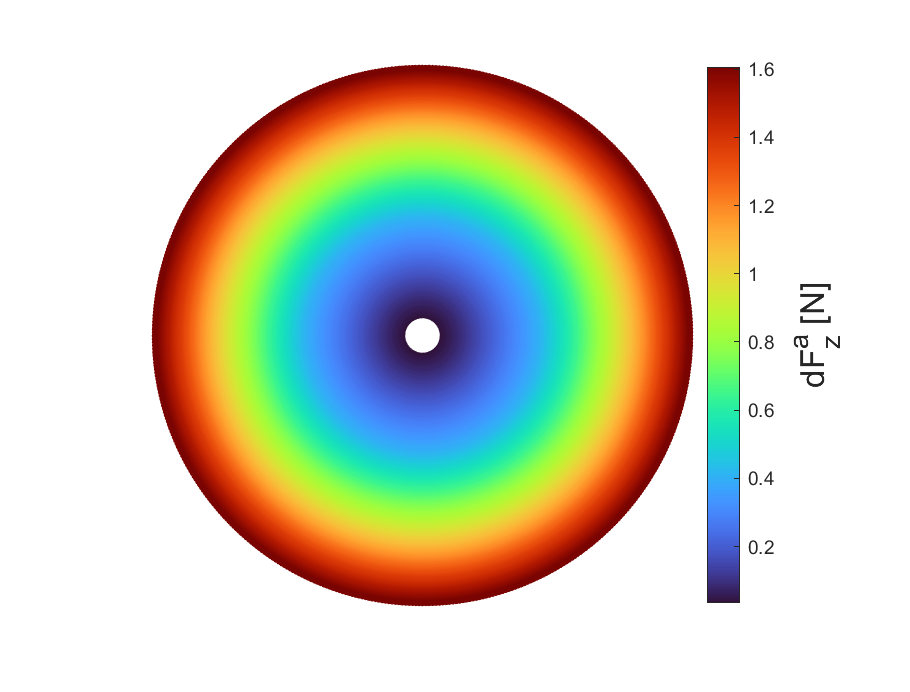
\includegraphics[width=0.49\textwidth]{Figures/comp_method/sim_B/dFz_a.eps}
    \caption{Axial force component $F_z$ in the aerodynamic reference frame}
    \label{fig:axial_force_paper}
\end{figure}

\begin{figure}[!htb]
    \centering
    \begin{minipage}{.49\textwidth}
      \centering
      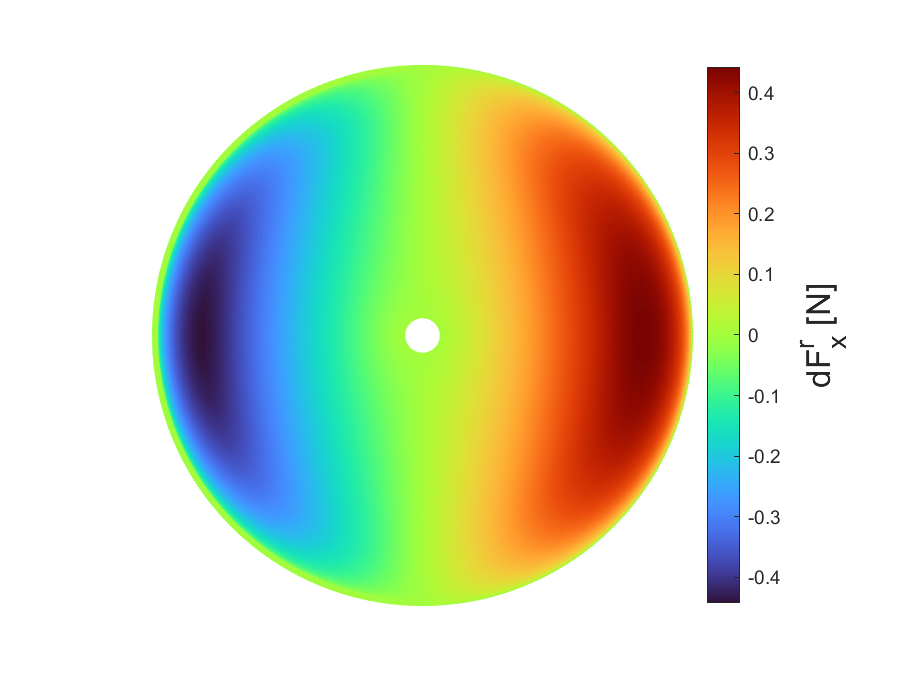
\includegraphics[width=\textwidth]{Figures/comp_method/sim_B/dFx_r.eps}
      \caption{Radial force component $F_x$ in the rotor reference frame}
      \label{fig:radial_force_rotor_paper}
    \end{minipage}%
    \hfill
    \begin{minipage}{.49\textwidth}
      \centering
      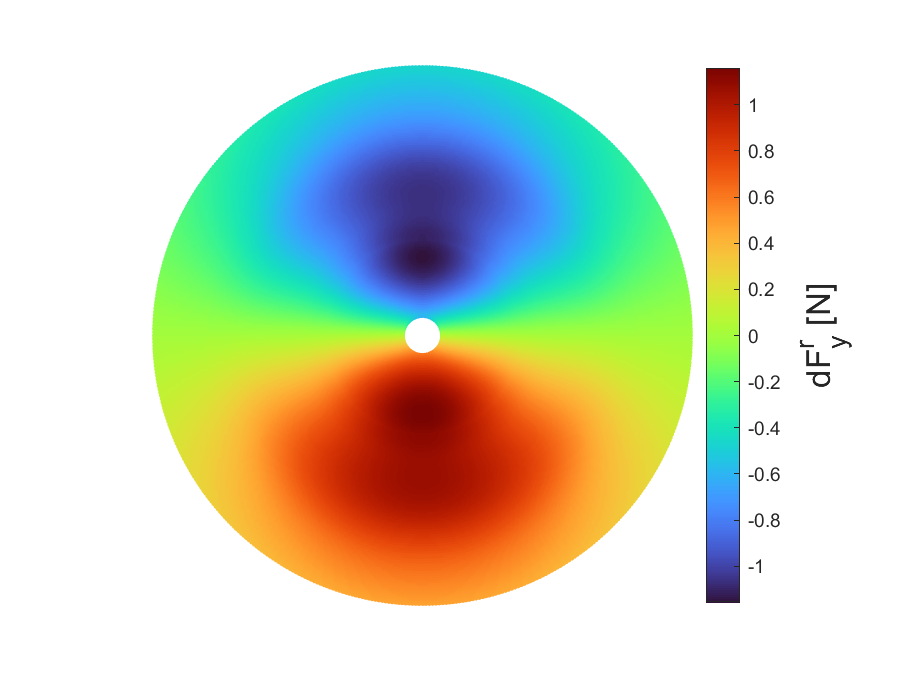
\includegraphics[width=\textwidth]{Figures/comp_method/sim_B/dFy_r.eps}
      \caption{Tangential force component $F_y$ in the rotor reference frame}
      \label{fig:tangential_force_rotor_paper}
    \end{minipage}
\end{figure}

\begin{figure}[!htb]
    \centering
    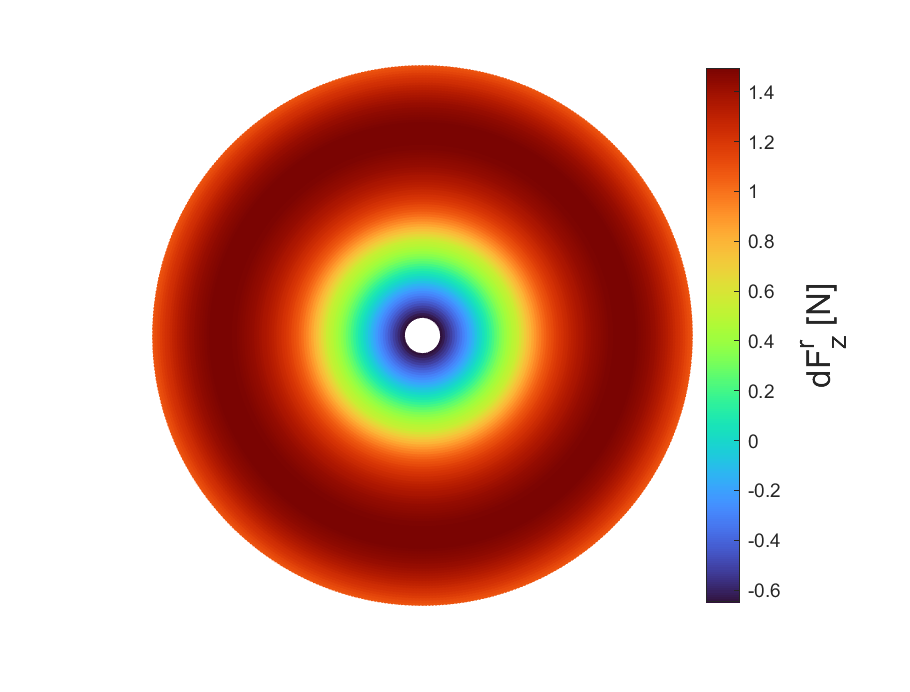
\includegraphics[width=0.49\textwidth]{Figures/comp_method/sim_B/dFz_r.eps}
    \caption{Axial force component $F_z$ in the rotor reference frame}
    \label{fig:axial_force_rotor_paper}
\end{figure}

\subsection{Descent with Forward Velocity Verification}


\subsection{Project Daedalus}


\subsection{Previous Work Comparison}


\section{Mesh Study}
\label{sec:mesh_study}

\subsection{Time Step}

\subsection{Rotor Mesh Discretization}

On this section, the mesh study is presented where three key points are discussed: 1) the time step for the dynamic model solver, 2) the azimutal rotor's distribution and 3) the blade element discretization for \gls{bet}.